\section{Validação}

Falar que vai ser feito uma pesquisa comparativa sobre o uso da ferramenta como solução de desacoplamento entre cliente e servidor em mudanças feitas no fluxo de dados pelo servidor. Para isso será desenvolvido um dois clientes para realizar 3 consultas em uma API REST, um fazendo o uso da ferramenta e o outro não. Após disso, aplicaremos uma série de mudanças no fluxo e analisaremos o resultado das variáveis coletadas. \\

\textbf{Estrutura de Dados (Entidades)} \\

Antes de realizar mudanças no fluxo, será preciso entender a estrutura de dados e os relacionamentos disponíveis no servidor no qual os clientes vão fazer consultas. Para isso, será usado uma implementação já disponível pela comunidade com o objetivo de testar implementações e estilos de arquiteturas para API web. Esta aplicação é baseado em entidades/dados da saga de filmes Starwars. As entidades apresentadas são: Filme, Pessoa, Espécie, Planeta, Espaçonave, Veículo. A seguir está um grafo para demonstrar o relacionamento entre eles.

\begin{figure}[H]
  \centering
  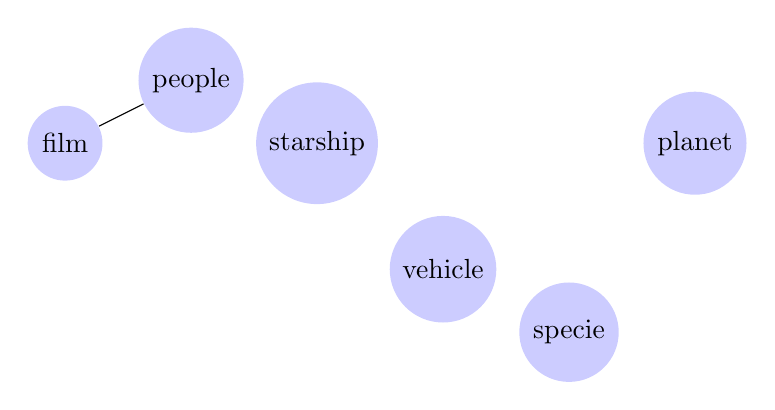
\begin{tikzpicture}
    [scale=.8,auto=left,every node/.style={circle,fill=blue!20}]
    \node (film) at (0,8)  {film};
    \node (people) at (2,9)  {people};
    \node (starship) at (4,8) {starship};
    \node (vehicle) at (6,6)  {vehicle};
    \node (specie) at (8,5)  {specie};
    \node (planet) at (10,8)  {planet};
    \foreach \from/\to in {people/film}
      \draw (\from) -- (\to);
  \end{tikzpicture}
  \caption{Entidades Starwars API (SWAPI)}
\end{figure}

\textbf{Consultas e respostas esperadas (Cliente)} \\

Para explorar bem todos os pontos de acesso da SWAPI. Foram pensadas 3 consultas de média complexidade que envolvessem pelo menos 3 das entidades descritas pela API. Para cada uma existe apenas uma resposta exata, onde é baseado nas estruturas de dados representes da API.

\begin{enumerate}
\item Qual o nome do filme no qual aparece mais personagens oriundos de um planeta deserto? R: "Revenge of the Sith"

\begin{figure}[H]
  \centering
  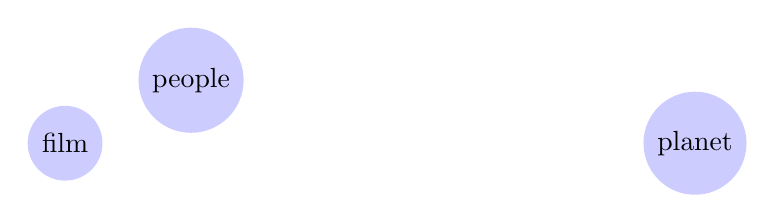
\begin{tikzpicture}
    [scale=.8,auto=left,every node/.style={circle,fill=blue!20}]
    \node (film) at (0,8)  {film};
    \node (people) at (2,9)  {people};
    \node (planet) at (10,8)  {planet};
  \end{tikzpicture}
  \caption{Entidades envolvidas na primeira pergunta}
\end{figure}

\item Qual o nome da espécie predominante entre os habitantes do planeta "Tatooine"? R: "Droid"

\begin{figure}[H]
  \centering
  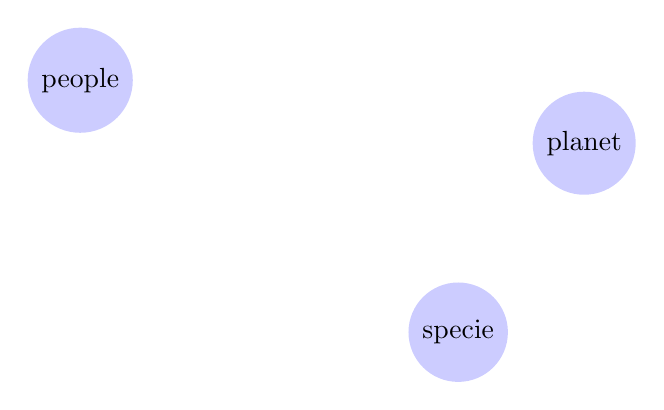
\begin{tikzpicture}
    [scale=.8,auto=left,every node/.style={circle,fill=blue!20}]
    \node (people) at (2,9)  {people};
    \node (specie) at (8,5)  {specie};
    \node (planet) at (10,8)  {planet};
  \end{tikzpicture}
  \caption{Entidades envolvidas na segunda pergunta}
\end{figure}

\item Qual o nome do personagem que mais pilota espaçonaves e veículos durante o filme "A New Hope"? R: "Chewbacca"

\begin{figure}[H]
  \centering
  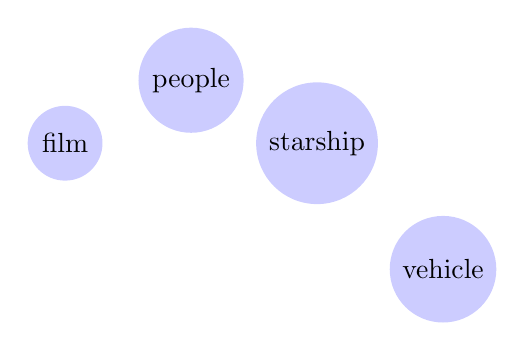
\begin{tikzpicture}
    [scale=.8,auto=left,every node/.style={circle,fill=blue!20}]
    \node (film) at (0,8)  {film};
    \node (people) at (2,9)  {people};
    \node (starship) at (4,8) {starship};
    \node (vehicle) at (6,6)  {vehicle};
  \end{tikzpicture}
  \caption{Entidades envolvidas na terceira pergunta}
\end{figure}

\end{enumerate}

\textbf{Mudanças no fluxo de dados (Servidor)} \\

Falar sobre os 3 tipos de mudanças. Primeiro é realocação, onde são pequenas mudanças no acesso. O segundo é transição, onde são considerados grandes mudanças como versionamento ou estilo de arquitetura. Por fim, o tipo de composição, onde o fluxo de dados é quebrado em diferentes serviços para separação de responsabilidades. Dizer que serão realizados 7 mudanças no fluxo de acesso da API REST (SWAPI) e comparado o impacto nos clientes.

\begin{description}[leftmargin=8em,style=nextline]
  \item[\textbf{Realocação}] 
  \begin{enumerate}
  \item Mudança no endereço de ponto de acesso.
  \item Mudança no nível de estrutura de resposta.
  \item Adição de ponto de acesso otimizado.
  \item Remoção de ponto de acesso deprecado.
  \end{enumerate}
  \item[\textbf{Transição}] 
  \begin{enumerate}
  \item[5.] Mudança de versão.
  \item[6.] Mudança no estilo de arquitetura.
  \end{enumerate}
  \item[\textbf{Composição}]
  \begin{enumerate}
  \item[7.] Mudança para micro-serviços.
  \end{enumerate}
\end{description}

Vale lembrar que nem todos os estilos de arquiteturas são vulneráveis a esses 3 tipos de mudanças. GraphQL por exemplo é desenvolvido para evitar mudanças de realocação, pois possuem apenas um acesso. Já REST, dependendo da sua implementação, está suscetível aos três. \\

\textbf{Variáveis} \\

Foram descritas treze variáveis para análise. doze delas quantitativas e uma delas qualitativa. Variáveis com o sufixo ** representam após a mudança. As variáveis que envolvem código referem-se ao código do cliente. Já o tamanho é considerado o código levado para configurar, buscar os dados e processar a resposta.

\begin{table}[H]
  \centering
  \begin{tabular}{|c|c|c|}
    \hline
    Variável & Unidade & Tipo \\
    \hline
    Tamanho do código & kb & Quantitativa \\
    \hline
    Tempo de resposta & ms & Quantitativa \\
    \hline
    Tamanho da resposta & kb & Quantitativa \\
    \hline
    Contagem de Requisição & inteiro & Quantitativa \\
    \hline
    Tempo de processamento & ms & Quantitativa \\
    \hline
    Buscou dados? ** & sim/não & Qualitativa \\
    \hline
    Tamanho do código ** & kb & Quantitativa \\
    \hline
    Tempo de resposta ** & ms & Quantitativa \\
    \hline
    Tamanho da resposta ** & kb & Quantitativa \\
    \hline
    Contagem de Requisição ** & inteiro & Quantitativa \\
    \hline
    Tempo de overhead ** & ms & Quantitativa \\
    \hline
  	Código adicionado ** & kb & Quantitativa \\
    \hline
  	Código removido ** & kb & Quantitativa \\
    \hline
  \end{tabular}
  \caption{Variáveis de validação}
\end{table}

 
 
 
 
 
 

 
